\documentclass[a4paper]{scrartcl}

\usepackage[
typ=ib,
fach=Mathematik,
lerngruppe=2BF,
farbig,
namensfeldAnzeigen,
datumAnzeigen,
seitenzahlen = auto,
loesungen = seite,
module= {Papiertypen}
]{schule}


\usepackage{amsmath}
\usepackage{float}
\usepackage[]{fourier-otf}
\usepackage{microtype}	
\author{Maximilian Hertenstein}
\date{\today}
\title{Geraden-Achsenschnittpunkte}
\date{Datum: \hspace{1.5cm}}

\usepackage{tkz-base}
\usepackage{tkz-fct}
\usepackage{tkz-euclide}
\ifoot{% TODO: \usepackage{graphicx} required

		
\includegraphics[width=0.3\linewidth]{GHSE-Logo}

}

\begin{document}




\begin{minipage}{0.5\linewidth}
\begin{center}
	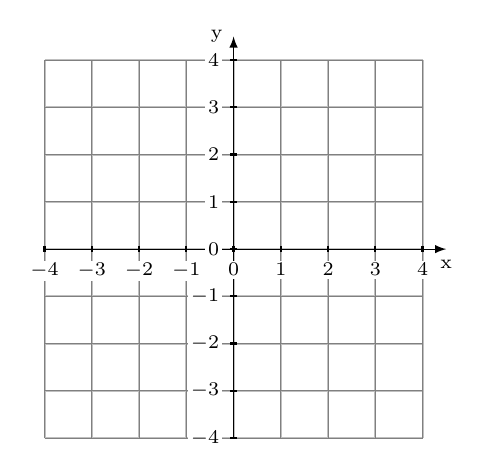
\begin{tikzpicture}[scale=.6]
		\scriptsize
		\tkzInit[ymax=4, xmax=4, xmin=-4, ymin=-4, xstep=1, ystep=1]
		\tkzGrid[sub,subxstep=1,subystep=1]
		\tkzFct[samples=50,domain=-5:5]{2*x-4}
		\tkzAxeXY[/tkzdrawX/label=x,/tkzdrawY/label=y]
	\end{tikzpicture}

\begin{center}
\begin{tabular}{|c|c|c|c|c|}
\hline
$x$ & $0$ & $1$ & $2$ & $3$  \\
\hline
$y$ & $$ & $$ & $$ & $$  \\
\hline
\end{tabular}
\end{center}

$$f: y = $$

\end{center}
\end{minipage}
\begin{minipage}{0.5\linewidth}
\begin{center}
	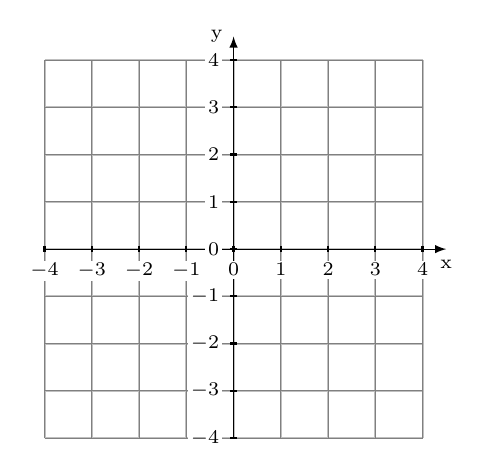
\begin{tikzpicture}[scale=.6]
		\scriptsize
		\tkzInit[ymax=4, xmax=4, xmin=-4, ymin=-4, xstep=1, ystep=1]
		\tkzGrid[sub,subxstep=1,subystep=1]
		\tkzFct[samples=50,domain=-5:5]{3-x}
		\tkzAxeXY[/tkzdrawX/label=x,/tkzdrawY/label=y]
	\end{tikzpicture}

\begin{center}
\begin{tabular}{|c|c|c|c|c|}
\hline
$x$ & $0$ & $1$ & $2$ & $3$  \\
\hline
$y$ & $$ & $$ & $$ & $$  \\
\hline
\end{tabular}
\end{center}

$$g: y = $$

\end{center}
\end{minipage}


\section{Schnittpunk mit y-Achse}
Den Schnittpunk mit der y-Achse kann man einfach aus der Geradengleichung ablesen.

\begin{minipage}{0.5\linewidth}


$$S_y = $$

\end{minipage}
\begin{minipage}{0.5\linewidth}




$$S_y = $$

\end{minipage}


\section{Schnittpunk mit x-Achse}
Die $y$-Koordinate des Schnittpunkts mit der x-Achse ist immer $\qquad$.
Die $x$-Koordinate erhält man durch Einsetzen von $y = 0$ in der Geradengleichung und Lösen der Gleichung.

\begin{minipage}{0.5\linewidth}

\feldKar{10}
$$S_x = $$

\end{minipage}
\begin{minipage}{0.5\linewidth}




\feldKar{10}
$$S_x = $$

\end{minipage}






\end{document} 